\documentclass{standalone}
\usepackage{pgf,tikz}
\usepackage{pgfplots}
%\usepackage{mathrsfs}
\usetikzlibrary{arrows}
\pagestyle{empty}
\begin{document}

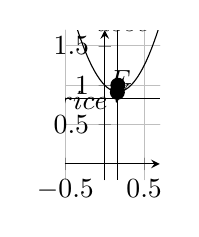
\begin{tikzpicture}[line cap=round,line join=round,>=triangle 45,x=1.0cm,y=1.0cm]
\begin{axis}[
x=1.0cm,y=1.0cm,
axis lines=middle,
ymajorgrids=true,
xmajorgrids=true,
xmin=-0.5,
xmax=0.7,
ymin=-0.2,
ymax=1.7,
]
\clip(-0.5,-0.2) rectangle (0.7,1.7);
\draw[color=black,smooth,samples=500,domain=-0.5:0.7] plot(\x,{3.0*(\x)^(2.0)-(\x)+1.0});
\draw  (0.16666666666666666,-0.2) -- (0.16666666666666666,1.7);
\draw [domain=-0.5:0.7] plot(\x,{(--0.8333333333333334-0.*\x)/1.});
\begin{scriptsize}

\draw (0.23389218325829664,1.7523488638482143) node {$asse$};
\draw [fill=black] (0.16666666666666666,1.) circle (2.5pt);
\draw (0.19199352553477722,1.064512566220439) node {$F$};
\draw [fill=black] (0.16057,0.91) circle (2.5pt);
\draw (0.20595974477595033,0.9004094901366552) node {$V$};
\draw (-0.771675602106169,0.80962906506903) node {$Direttrice$};
\end{scriptsize}
\end{axis}
\end{tikzpicture}
\end{document}